% Options for packages loaded elsewhere
% Options for packages loaded elsewhere
\PassOptionsToPackage{unicode}{hyperref}
\PassOptionsToPackage{hyphens}{url}
%
\documentclass[
  11pt,
  letterpaper,
  DIV=11,
  numbers=noendperiod,
  twoside]{scrartcl}
\usepackage{xcolor}
\usepackage[left=1.1in, right=1in, top=0.8in, bottom=0.8in,
paperheight=9.5in, paperwidth=7in, includemp=TRUE, marginparwidth=0in,
marginparsep=0in]{geometry}
\usepackage{amsmath,amssymb}
\setcounter{secnumdepth}{3}
\usepackage{iftex}
\ifPDFTeX
  \usepackage[T1]{fontenc}
  \usepackage[utf8]{inputenc}
  \usepackage{textcomp} % provide euro and other symbols
\else % if luatex or xetex
  \usepackage{unicode-math} % this also loads fontspec
  \defaultfontfeatures{Scale=MatchLowercase}
  \defaultfontfeatures[\rmfamily]{Ligatures=TeX,Scale=1}
\fi
\usepackage{lmodern}
\ifPDFTeX\else
  % xetex/luatex font selection
  \setmainfont[ItalicFont=EB Garamond Italic,BoldFont=EB Garamond
SemiBold]{EB Garamond Math}
  \setsansfont[]{EB Garamond}
  \setmathfont[]{Garamond-Math}
\fi
% Use upquote if available, for straight quotes in verbatim environments
\IfFileExists{upquote.sty}{\usepackage{upquote}}{}
\IfFileExists{microtype.sty}{% use microtype if available
  \usepackage[]{microtype}
  \UseMicrotypeSet[protrusion]{basicmath} % disable protrusion for tt fonts
}{}
\usepackage{setspace}
% Make \paragraph and \subparagraph free-standing
\makeatletter
\ifx\paragraph\undefined\else
  \let\oldparagraph\paragraph
  \renewcommand{\paragraph}{
    \@ifstar
      \xxxParagraphStar
      \xxxParagraphNoStar
  }
  \newcommand{\xxxParagraphStar}[1]{\oldparagraph*{#1}\mbox{}}
  \newcommand{\xxxParagraphNoStar}[1]{\oldparagraph{#1}\mbox{}}
\fi
\ifx\subparagraph\undefined\else
  \let\oldsubparagraph\subparagraph
  \renewcommand{\subparagraph}{
    \@ifstar
      \xxxSubParagraphStar
      \xxxSubParagraphNoStar
  }
  \newcommand{\xxxSubParagraphStar}[1]{\oldsubparagraph*{#1}\mbox{}}
  \newcommand{\xxxSubParagraphNoStar}[1]{\oldsubparagraph{#1}\mbox{}}
\fi
\makeatother


\usepackage{longtable,booktabs,array}
\usepackage{calc} % for calculating minipage widths
% Correct order of tables after \paragraph or \subparagraph
\usepackage{etoolbox}
\makeatletter
\patchcmd\longtable{\par}{\if@noskipsec\mbox{}\fi\par}{}{}
\makeatother
% Allow footnotes in longtable head/foot
\IfFileExists{footnotehyper.sty}{\usepackage{footnotehyper}}{\usepackage{footnote}}
\makesavenoteenv{longtable}
\usepackage{graphicx}
\makeatletter
\newsavebox\pandoc@box
\newcommand*\pandocbounded[1]{% scales image to fit in text height/width
  \sbox\pandoc@box{#1}%
  \Gscale@div\@tempa{\textheight}{\dimexpr\ht\pandoc@box+\dp\pandoc@box\relax}%
  \Gscale@div\@tempb{\linewidth}{\wd\pandoc@box}%
  \ifdim\@tempb\p@<\@tempa\p@\let\@tempa\@tempb\fi% select the smaller of both
  \ifdim\@tempa\p@<\p@\scalebox{\@tempa}{\usebox\pandoc@box}%
  \else\usebox{\pandoc@box}%
  \fi%
}
% Set default figure placement to htbp
\def\fps@figure{htbp}
\makeatother


% definitions for citeproc citations
\NewDocumentCommand\citeproctext{}{}
\NewDocumentCommand\citeproc{mm}{%
  \begingroup\def\citeproctext{#2}\cite{#1}\endgroup}
\makeatletter
 % allow citations to break across lines
 \let\@cite@ofmt\@firstofone
 % avoid brackets around text for \cite:
 \def\@biblabel#1{}
 \def\@cite#1#2{{#1\if@tempswa , #2\fi}}
\makeatother
\newlength{\cslhangindent}
\setlength{\cslhangindent}{1.5em}
\newlength{\csllabelwidth}
\setlength{\csllabelwidth}{3em}
\newenvironment{CSLReferences}[2] % #1 hanging-indent, #2 entry-spacing
 {\begin{list}{}{%
  \setlength{\itemindent}{0pt}
  \setlength{\leftmargin}{0pt}
  \setlength{\parsep}{0pt}
  % turn on hanging indent if param 1 is 1
  \ifodd #1
   \setlength{\leftmargin}{\cslhangindent}
   \setlength{\itemindent}{-1\cslhangindent}
  \fi
  % set entry spacing
  \setlength{\itemsep}{#2\baselineskip}}}
 {\end{list}}
\usepackage{calc}
\newcommand{\CSLBlock}[1]{\hfill\break\parbox[t]{\linewidth}{\strut\ignorespaces#1\strut}}
\newcommand{\CSLLeftMargin}[1]{\parbox[t]{\csllabelwidth}{\strut#1\strut}}
\newcommand{\CSLRightInline}[1]{\parbox[t]{\linewidth - \csllabelwidth}{\strut#1\strut}}
\newcommand{\CSLIndent}[1]{\hspace{\cslhangindent}#1}



\setlength{\emergencystretch}{3em} % prevent overfull lines

\providecommand{\tightlist}{%
  \setlength{\itemsep}{0pt}\setlength{\parskip}{0pt}}



 


\setlength\heavyrulewidth{0ex}
\setlength\lightrulewidth{0ex}
\usepackage[automark]{scrlayer-scrpage}
\clearpairofpagestyles
\cehead{
  Brian Weatherson
  }
\cohead{
  The End of Decision Theory
  }
\ohead{\bfseries \pagemark}
\cfoot{}
\makeatletter
\newcommand*\NoIndentAfterEnv[1]{%
  \AfterEndEnvironment{#1}{\par\@afterindentfalse\@afterheading}}
\makeatother
\NoIndentAfterEnv{itemize}
\NoIndentAfterEnv{enumerate}
\NoIndentAfterEnv{description}
\NoIndentAfterEnv{quote}
\NoIndentAfterEnv{equation}
\NoIndentAfterEnv{longtable}
\NoIndentAfterEnv{abstract}
\renewenvironment{abstract}
 {\vspace{-1.25cm}
 \quotation\small\noindent\emph{Abstract}:}
 {\endquotation}
\newfontfamily\tfont{EB Garamond}
\addtokomafont{disposition}{\rmfamily}
\addtokomafont{title}{\normalfont\itshape}
\let\footnoterule\relax

\makeatletter
\renewcommand{\@maketitle}{%
  \newpage
  \null
  \vskip 2em%
  \begin{center}%
  \let \footnote \thanks
    {\itshape\huge\@title \par}%
    \vskip 0.5em%  % Reduced from default
    {\large
      \lineskip 0.3em%  % Reduced from default 0.5em
      \begin{tabular}[t]{c}%
        \@author
      \end{tabular}\par}%
    \vskip 0.5em%  % Reduced from default
    {\large \@date}%
  \end{center}%
  \par
  }
\makeatother
\RequirePackage{lettrine}

\renewenvironment{abstract}
 {\quotation\small\noindent\emph{Abstract}:}
 {\endquotation\vspace{-0.02cm}}
\KOMAoption{captions}{tableheading}
\makeatletter
\@ifpackageloaded{caption}{}{\usepackage{caption}}
\AtBeginDocument{%
\ifdefined\contentsname
  \renewcommand*\contentsname{Table of contents}
\else
  \newcommand\contentsname{Table of contents}
\fi
\ifdefined\listfigurename
  \renewcommand*\listfigurename{List of Figures}
\else
  \newcommand\listfigurename{List of Figures}
\fi
\ifdefined\listtablename
  \renewcommand*\listtablename{List of Tables}
\else
  \newcommand\listtablename{List of Tables}
\fi
\ifdefined\figurename
  \renewcommand*\figurename{Figure}
\else
  \newcommand\figurename{Figure}
\fi
\ifdefined\tablename
  \renewcommand*\tablename{Table}
\else
  \newcommand\tablename{Table}
\fi
}
\@ifpackageloaded{float}{}{\usepackage{float}}
\floatstyle{ruled}
\@ifundefined{c@chapter}{\newfloat{codelisting}{h}{lop}}{\newfloat{codelisting}{h}{lop}[chapter]}
\floatname{codelisting}{Listing}
\newcommand*\listoflistings{\listof{codelisting}{List of Listings}}
\makeatother
\makeatletter
\makeatother
\makeatletter
\@ifpackageloaded{caption}{}{\usepackage{caption}}
\@ifpackageloaded{subcaption}{}{\usepackage{subcaption}}
\makeatother
\usepackage{bookmark}
\IfFileExists{xurl.sty}{\usepackage{xurl}}{} % add URL line breaks if available
\urlstyle{same}
\hypersetup{
  pdftitle={The End of Decision Theory},
  pdfauthor={Brian Weatherson},
  hidelinks,
  pdfcreator={LaTeX via pandoc}}


\title{The End of Decision Theory}
\author{Brian Weatherson}
\date{2025}
\begin{document}
\maketitle
\begin{abstract}
What question are decision theorists trying to answer, and why is it
worth trying to answer it? A lot of philosophers talk as if the aim of
decision theory is to describe how we should make decisions, and the
reason to do this is to help us make better decisions. I disagree on
both fronts. The aim of the decision theory is to describe how a certain
kind of idealised decider does in fact decide. And the reason to do this
is that this idealisation, like many other idealisations, helps generate
explanations of real-world behaviour. We shouldn't do what these ideal
deciders do, or try to be more like them, because a lot of what they do
only makes sense because of the differences between us and them. Still,
sometimes those differences are small enough that they can be ignored in
explanations, and that's when decision theory is useful.
\end{abstract}


\setstretch{1.1}
What are philosophical decision theorists trying to do? A simple answer
is that they are trying to find the correct decision theory. This
invites two more questions. What does it mean to say some decision
theory is correct? And why should we care about knowing which one is
correct?

I think most decision theorists would endorse some kind of normative
answer to these questions. The correct decision theory is the one that
agents, or at least a certain kind of agent, should follow. We should
figure out what it is so we can advise agents on how to make better
decisions.

This paper argues against this normative answer, and in favor of a
descriptive answer. The correct decision theory is one that accurately
describes what a certain kind of agent will do. Finding the correct
answer is useful because it helps us explain certain patterns of
behavior, especially in highly social settings.

The descriptive answer might seem obviously false in light of the fact
that decision theory is quite clearly about idealised agents. The
important point to note here that we use `idealised' in philosophy (and
academia more generally) in two rather distinct ways.\footnote{This
  ambiguity in the term `idealised' is also noted in Carr, Greco, and
  Roussos.} In political philosophy, when people talk about ideal
theory, they are talking about some kind of optimum. This sense is
clearly normative. But in much of philosophy of science, we talk about
ideals in a purely descriptive way. An idealised model need not be
better than reality. The ideal gases in the ideal gas model are not
better in virtue of having point sized molecules. Size is not a failure
that we imagine gases sloughing off. I'm going to argue that the ideal
agents in ideal decision theory are more like ideal gases than they are
like ideal states.

While this is an ambiguity, you might think that the meanings are not
incompatible. The ideal agents in decision theory might be both optima
and simplifications. Indeed, I think that in a good sense they are.
Still, I'll argue, we should take the simplification sense to be more
central. What's important about these idealised agents is that they can
play a role in what I'll call strongly reflexive explanations of social
phenomena. These are explanations where the agents involved not just
realise that the explanation in question correctly describes their
situation, but do what they do in part because of this realisation. Such
explanations work most smoothly when the explanatory models are not just
simplifications of real life, but also involve some kind of optimal
behavior.

\section{Two Cases}\label{two-cases}

I'm interested in philosophical decision theory\footnote{I'll treat the
  modifier `philosophical' as understood from here on.} as it's
currently practiced. So I'll start with two cases that every theory on
the market agrees about.\footnote{In recent years decision theorists
  have focussed on two big questions. One is whether the ideal agent
  could be risk-sensitive. Lara Buchak (\citeproc{ref-BuchakRisk}{2013})
  argues for yes, and her position has been criticised by, inter alia,
  Ray Briggs (\citeproc{ref-Briggs2015}{2015}) and Joanna Thoma
  (\citeproc{ref-Thoma2019}{2019}). The other is how the ideal agent
  handles Newcomb-like problems, broadly construed. A traditional
  version of the one-box answer is defended by Arif Ahmed
  (\citeproc{ref-Ahmed2014}{2014}); a more radical kind of one-boxing by
  Ben Levinstein and Nate Soares
  (\citeproc{ref-LevinsteinSoares2020}{2020}). There are a flood of
  variants of two-boxing, each pair of which disagree on some case or
  other. Such theories have been put forward by William Harper
  (\citeproc{ref-Harper1986}{1986}), James Joyce
  (\citeproc{ref-Joyce1999}{1999}), Frank Arntzenius
  (\citeproc{ref-Arntzenius2008}{2008}), Johan Gustafsson
  (\citeproc{ref-Gustafsson2011}{2011}), Ralph Wedgwood
  (\citeproc{ref-Wedgwood2013a}{2013}), Dmitri Gallow
  (\citeproc{ref-Gallow2020}{2020}), Abelard Podgorski
  (\citeproc{ref-Podgorski2022}{2022}), David Barnett
  (\citeproc{ref-Barnett2022}{2022}), Jack Spencer
  (\citeproc{ref-Spencer2023}{2023}) and Melissa Fusco
  (\citeproc{ref-Fuscond}{n.d.}). The arguments I'll make here are
  strictly speaking between these views, but they fit most smoothly with
  Harper and Fusco's views.} These provide an important pair of
constraints. Whatever the correct decision theory is, it must be one
that agrees on these cases.

\subsection{Betting}\label{betting}

Chooser has \$110, and is in a sports betting shop. There is a
basketball game about to start, between two teams they know to be
equally matched. Chooser has three options: bet the \$110 on Home, bet
it on Away, keep money. If they bet and are right, they win \$100 (plus
get the money back they bet), if they are wrong, they lose the money.
Given standard assumptions about how much Chooser likes money, all the
decision theories I'm discussing say Chooser should not bet.

From this it follows that decision theory is not in the business of
answering this question: \emph{What action will produce the best
outcome?}. We know, and so does Chooser, that the action that produces
the best outcome is to bet on the winning team. Keeping their money in
their pocket is the only action they know will be sub-optimal. And it's
what decision theory says to do.

This is to say, decision theory is not axiology. It's not a theory of
evaluating outcomes, and saying which is best. Axiology is a very
important part of philosophy, but it's not what decision theorists are
up to.

So far this will probably strike you, dear reader, as obvious. But
there's another step, that I think will strike some people as nearly as
obvious, that I'm at pains to resist. Some might say that decision
theorists don't tell Chooser to bet on the winner because this is lousy
advice. Chooser can't bet on the winner, at least not as such. That,
I'll argue, would be a misstep. Decision theorists do not restrict
themselves to answers that can be practically carried out.

\subsection{Salesman}\label{salesman}

We'll focus on a version of what Julia Robinson
(\citeproc{ref-Robinson1949}{1949}) called the travelling salesman
problem.\footnote{For a thorough history of the problem, see Schrijver
  (\citeproc{ref-Schrijver2005}{2005}). For an accessible history of the
  problem, which includes these references, see Travelling salesman
  problem (\citeproc{ref-wiki-salesman}{2024}).} Given some points on a
map, find the shortest path through them. We'll focus on the 257 cities
shown on the map in Figure~\ref{fig-map}.

\begin{figure}

\centering{

\pandocbounded{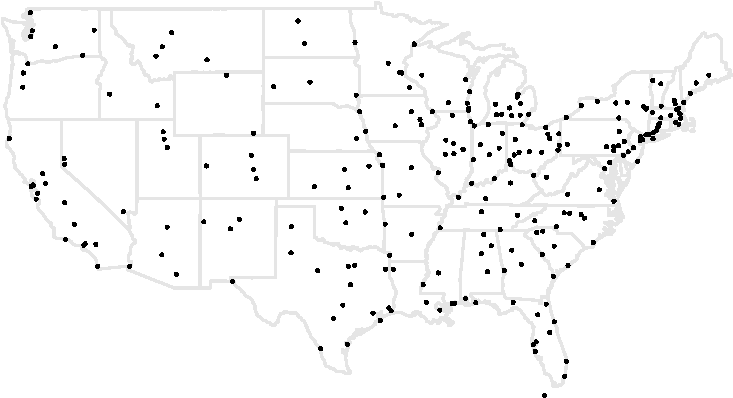
\includegraphics[keepaspectratio]{dec-2024-draft_files/figure-pdf/fig-map-1.pdf}}

}

\caption{\label{fig-map}257 American cites; our task is to find the
shortest path that goes through all of them.}

\end{figure}%

The task is to find the shortest path through those 257
cities.\footnote{The 257 cities are the cities in the lower 48 states
  from the 312 cities in North America that John Burkardt
  (\citeproc{ref-Burkhart2011}{2011}) mapped in his dataset USCA312.}

All decision theories on the market say the thing to do here is to draw
whichever of the 256! possible paths is shortest. That is not
particularly helpful advice. Unless you know a lot about problems like
this, you can't draw the shortest path through the map. And least, you
can't draw it as such. You can't draw it in the way that you can't enter
the correct code on a locked phone
(\citeproc{ref-MandelkernEtAl2017}{Mandelkern, Schultheis, and Boylan
2017}).

If one wanted to give advice about puzzles like this, there is a lot to
say. For people with access to typical amounts of computing power, e.g.,
the amount of power the computer I'm writing this on has, and who don't
lose a lot by choosing a path a little longer than optimal, it's helpful
to advise them to use a Farthest Insertion Algorithm.\footnote{The
  algorithm is described in the documentation of the TSP package by
  Michael Hashler and Kurt Hornik
  (\citeproc{ref-HashlerHornik2007}{2007}). I used that package to
  implement the algorithm and also to find the two shorter maps that
  follow.} Figure~\ref{fig-farthest} shows the result of one output of
this algorithm.\footnote{The algorithm is silent on which city you start
  with, and usually chooses this randomly.}

\begin{figure}

\centering{

\pandocbounded{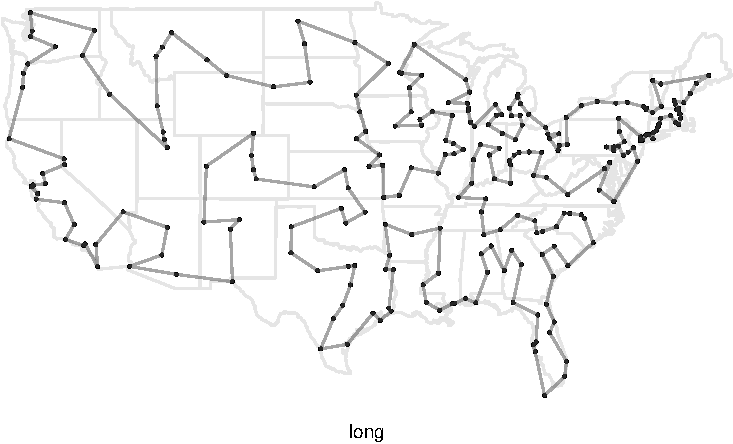
\includegraphics[keepaspectratio]{dec-2024-draft_files/figure-pdf/fig-farthest-1.pdf}}

}

\caption{\label{fig-farthest}An output of the Farthest Insertion
Algorithm, with a length of 21075 miles.}

\end{figure}%

If the advisee has a bit more power at hand, and cares a bit about fine
improvements, there are further algorithms you could suggest to them.
Some of these don't start with just the cities, but take an existing
path and find small improvements to it. One simple enough improvement
algorithm turns Figure~\ref{fig-farthest} into Figure~\ref{fig-two-opt}.

\begin{figure}

\centering{

\pandocbounded{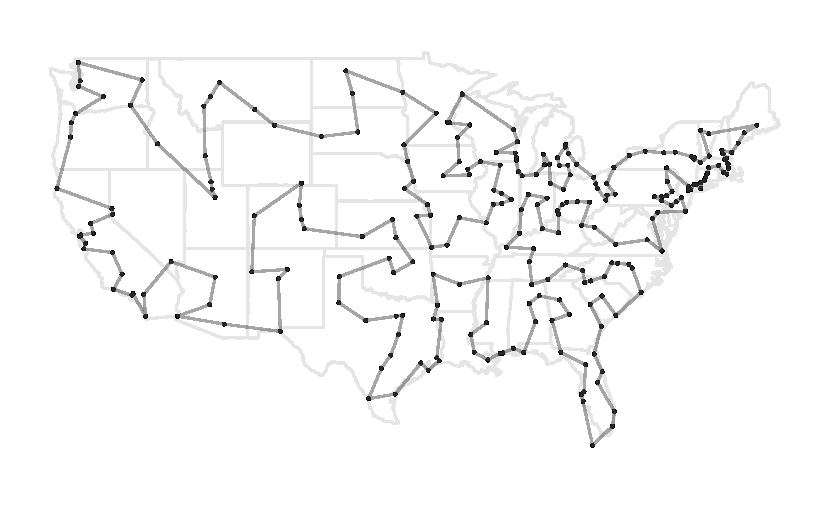
\includegraphics[keepaspectratio]{dec-2024-draft_files/figure-pdf/fig-two-opt-1.pdf}}

}

\caption{\label{fig-two-opt}The output of an optimisation process, which
reduced the path length to 20891 miles.}

\end{figure}%

Beyond this, you have to either really care about the path length, or
have quite a bit of time or computing power to spare. By a bit of brute
force, I found the path in Figure~\ref{fig-best}. I'm not sure it is
optimal, and the methods that got there aren't entirely scalable. It is,
however, about 3\% shorter than Figure~\ref{fig-farthest} and 2\%
shorter than Figure~\ref{fig-two-opt}.

\begin{figure}

\centering{

\pandocbounded{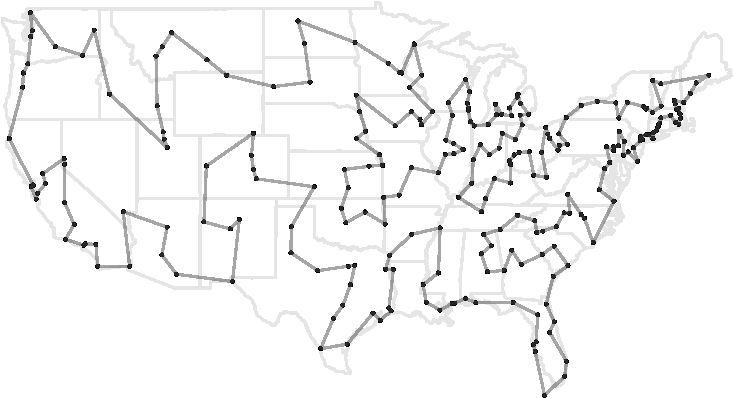
\includegraphics[keepaspectratio]{dec-2024-draft_files/figure-pdf/fig-best-1.pdf}}

}

\caption{\label{fig-best}The shortest path I could find, with a distance
of 20301 miles.}

\end{figure}%

\subsection{The Two Cases}\label{the-two-cases}

Table~\ref{tbl-examples} summarises the examples from the last two
subsections.

\begin{longtable}[]{@{}lcc@{}}
\caption{How three approaches to decision theory handle the two
cases}\label{tbl-examples}\tabularnewline
\toprule\noalign{}
& Betting & Salesman \\
\midrule\noalign{}
\endfirsthead
\toprule\noalign{}
& Betting & Salesman \\
\midrule\noalign{}
\endhead
\bottomrule\noalign{}
\endlastfoot
Best outcome & Bet on winner & Shortest path \\
Decision theory & Pass & Shortest path \\
Best advice & Pass & Learn algorithms \\
\end{longtable}

The first row says which action would produce the best outcome in the
two cases. The third row says what advice one ought give someone who had
to choose in the two cases. And the middle row says what all the
decision theories say about the two cases. Notably, it agrees with
neither the first nor third row. Decision theory is neither in the
business of saying what will produce the best result, nor with giving
the most useful advice. So what is it doing?

\phantomsection\label{refs}
\begin{CSLReferences}{1}{0}
\bibitem[\citeproctext]{ref-Ahmed2014}
Ahmed, Arif. 2014. \emph{Evidence, Decision and Causality}. Cambridge:
{C}ambridge {U}niversity {P}ress.

\bibitem[\citeproctext]{ref-Arntzenius2008}
Arntzenius, Frank. 2008. {``No Regrets; or, Edith Piaf Revamps Decision
Theory.''} \emph{Erkenntnis} 68 (2): 277--97. doi:
\href{https://doi.org/10.1007/s10670-007-9084-8}{10.1007/s10670-007-9084-8}.

\bibitem[\citeproctext]{ref-Barnett2022}
Barnett, David James. 2022. {``Graded Ratifiability.''} \emph{Journal of
Philosophy} 119 (2): 57--88. doi:
\href{https://doi.org/10.5840/jphil202211925}{10.5840/jphil202211925}.

\bibitem[\citeproctext]{ref-Briggs2015}
Briggs, Ray. 2015. {``Costs of Abandoning the Sure-Thing Principle.''}
\emph{Canadian Journal of Philosophy} 45 (5): 827--40. doi:
\href{https://doi.org/10.1080/00455091.2015.1122387}{10.1080/00455091.2015.1122387}.

\bibitem[\citeproctext]{ref-BuchakRisk}
Buchak, Lara. 2013. \emph{Risk and Rationality}. Oxford: Oxford
University Press.

\bibitem[\citeproctext]{ref-Burkhart2011}
Burkardt, John. 2011. {``Cities.''}
\url{https://people.sc.fsu.edu/~jburkardt/datasets/cities/cities.html}.

\bibitem[\citeproctext]{ref-Fuscond}
Fusco, Melissa. n.d. {``Absolution of a Causal Decision Theorist.''}
\emph{No{û}s}. doi:
\href{https://doi.org/10.1111/nous.12459}{10.1111/nous.12459}. Early
view.

\bibitem[\citeproctext]{ref-Gallow2020}
Gallow, J. Dmitri. 2020. {``The Causal Decision Theorist's Guide to
Managing the News.''} \emph{The Journal of Philosophy} 117 (3): 117--49.
doi:
\href{https://doi.org/10.5840/jphil202011739}{10.5840/jphil202011739}.

\bibitem[\citeproctext]{ref-Gustafsson2011}
Gustafsson, Johan E. 2011. {``A Note in Defence of Ratificationism.''}
\emph{Erkenntnis} 75 (1): 147--50. doi:
\href{https://doi.org/10.1007/s10670-010-9267-6}{10.1007/s10670-010-9267-6}.

\bibitem[\citeproctext]{ref-HashlerHornik2007}
Hahsler, Michael, and Kurt Hornik. 2007. {``TSP---Infrastructure for the
Traveling Salesperson Problem.''} \emph{Journal of Statistical Software}
23 (2): 1--21. doi:
\href{https://doi.org/10.18637/jss.v023.i02}{10.18637/jss.v023.i02}.

\bibitem[\citeproctext]{ref-Harper1986}
Harper, William. 1986. {``Mixed Strategies and Ratifiability in Causal
Decision Theory.''} \emph{Erkenntnis} 24 (1): 25--36. doi:
\href{https://doi.org/10.1007/BF00183199}{10.1007/BF00183199}.

\bibitem[\citeproctext]{ref-Joyce1999}
Joyce, James M. 1999. \emph{The Foundations of Causal Decision Theory}.
Cambridge: Cambridge University Press.

\bibitem[\citeproctext]{ref-LevinsteinSoares2020}
Levinstein, Benjamin Anders, and Nate Soares. 2020. {``Cheating Death in
Damascus.''} \emph{Journal of Philosophy} 117 (5): 237--66. doi:
\href{https://doi.org/10.5840/jphil2020117516}{10.5840/jphil2020117516}.

\bibitem[\citeproctext]{ref-MandelkernEtAl2017}
Mandelkern, Matthew, Ginger Schultheis, and David Boylan. 2017.
{``Agentive Modals.''} \emph{Philosophical Review} 126 (3): 301--43.
doi:
\href{https://doi.org/10.1215/00318108-3878483}{10.1215/00318108-3878483}.

\bibitem[\citeproctext]{ref-Podgorski2022}
Podgorski, Aberlard. 2022. {``Tournament Decision Theory.''}
\emph{No{û}s} 56 (1): 176--203. doi:
\href{https://doi.org/10.1111/nous.12353}{10.1111/nous.12353}.

\bibitem[\citeproctext]{ref-Robinson1949}
Robinson, Julia. 1949. {``On the Hamiltonian Game (a Traveling Salesman
Problem).''} Santa Monica, CA: The RAND Corporation.

\bibitem[\citeproctext]{ref-Schrijver2005}
Schrijver, Alexander. 2005. {``On the History of Combinatorial
Optimization (till 1960).''} \emph{Handbooks in Operations Research and
Management Science} 12: 1--68. doi:
\href{https://doi.org/10.1016/S0927-0507(05)12001-5}{10.1016/S0927-0507(05)12001-5}.

\bibitem[\citeproctext]{ref-Spencer2023}
Spencer, Jack. 2023. {``Can It Be Irrational to Knowingly Choose the
Best?''} \emph{Australasian Journal of Philosophy} 101 (1): 128--39.
doi:
\href{https://doi.org/10.1080/00048402.2021.1958880}{10.1080/00048402.2021.1958880}.

\bibitem[\citeproctext]{ref-Thoma2019}
Thoma, Johanna. 2019. {``Risk Aversion and the Long Run.''}
\emph{Ethics} 129 (2): 230--53. doi:
\href{https://doi.org/10.1086/699256}{10.1086/699256}.

\bibitem[\citeproctext]{ref-wiki-salesman}
Travelling salesman problem. 2024. {``Travelling Salesman Problem---
{W}ikipedia{,} the Free Encyclopedia.''}
\url{https://en.wikipedia.org/w/index.php?title=Travelling_salesman_problem&oldid=1209291065}.
{[}Online; accessed 27-February-2024{]}.

\bibitem[\citeproctext]{ref-Wedgwood2013a}
Wedgwood, Ralph. 2013. {``Gandalf's Solution to the Newcomb Problem.''}
\emph{Synthese} 190 (14): 2643--75. doi:
\href{https://doi.org/10.1007/s11229-011-9900-1}{10.1007/s11229-011-9900-1}.

\end{CSLReferences}



\noindent Unpublished. Posted online in 2024.


\end{document}
